\chapter{Controlador de corriente} \chapterlabel{Informe/4-ControladorCorriente} \label{cap:ControladorCorriente}

En este capítulo se diseña y modela el circuito encargado de controlar la corriente que circula por el electroimán. Como se vio en el capítulo anterior, El sistema trabaja con corrientes elevadas se implementan estrategias de conmutación para reducir las pérdidas de energía. Para ello se utiliza una topología de puente H con cuatro MOSFET y un \textsl{driver} que los controla. Además, se detallan los criterios tenidos en cuenta al momento de  elegir  y dimensionar todos los componentes que intervienen para lograr el correcto funcionamiento del controlador de corriente. Por último, se obtiene su función transferencia  para ser utilizada en el diseño del compensador.

\section{Descripción general}

\noindent Para regular la fuerza ejercida por el electroimán es necesario controlar la corriente que circula por él. Para ello, se modela a la planta como la admitancia de un circuito RL serie. En el capítulo \ref{cap:CaracterizacionElectroiman} se determinó que la inductancia varía con el entrehierro. Por lo tanto, la expresión resulta: 

\begin{equation} \label{eq_admitancia}
	\frac{1}{sL(Y_g)\ +\ R_L}
\end{equation}

\noindent Se desea controlar la corriente que circula por el electroimán y, debido a que el sistema va a trabajar con corrientes elevadas, es importante que la implementación del controlador de corriente sea eficiente. Por lo tanto, para disminuir la disipación de potencia del circuito se utiliza un controlador que funciona en conmutación. 

\noindent Para lograr una corriente contínua en el electroimán mediante una fuente conmutada se debe alternar la polaridad de la tensión aplicada en los bornes del inductor. De esta forma, la corriente crece y decrece (según la polaridad de tensión aplicada) con forma exponencial debido a la resistencia interna del electroimán. Sin embargo, como el intervalo de tiempo de esta conmutación es pequeño comparado con la constante de tiempo de la planta, el incremento de corriente será pequeño y puede ser aproximado a una recta. Por lo tanto, se obtiene una corriente contínua con un ripple superpuesto de forma triangular. 

\noindent Para lograr alternar la polaridad de la fuente sobre el inductor se utiliza una topología en puente H con cuatro llaves como se  muestra en la figura.\colorbox{red}{HACER IMAGEN CON LLAVES} 

El electroimán se conecta entre los puntos medios de cada par de llaves. De esta manera se puede conmutar la polaridad de la tensión que se le aplica. Sólo se permite que dos llaves se enciendan a la vez, y esto se realiza de manera diagonal. Es decir, en la figura \ref{fig:img_topologia-puenteH}, $Q_1$ y $Q_4$ pueden estar encendidos, mientras que $Q_3$ y $Q_2$ están apagados, y viceversa. De otra forma, se podría generar un cortocircuito entre la fuente de alimentación y GND, que produciría una circulación de corriente denominada \textsl{shoot-through}.

Para poder generar una corriente triangular con un valor medio deseado es necesario controlar el tiempo que se le aplica cierta polaridad de tensión al electroimán. Para poder controlar dicha polaridad, se debe actuar sobre las llaves en función de si se desea aumentar o disminuir el valor medio de la corriente.  Una manera de hacerlo es mediante un comparador con histéresis, cuya salida determina que llaves se encienden en función de comparar la corriente de referencia con la que está circulando por el electroimán. En caso de que esta última sea menor qeu la referencia, la polaridad de tensión aplicada al electroimán será positiva y, por ende, la corriente aumentara hasta alcanzar la referencia. Una vez superada la referencia, se volverá a cambiar la polaridad en el electoimán, pero esta vez será negativa, haciendo que el valor medio de la corriente disminuya. De esta forma, se puede observar que va a haber un riple en torno al valor medio de corriente deseado.  Este riple debe ser...



permanecen encendidas las llaves en 
Al controlar el tiempo de activación de las llaves, se podría obtener una forma de onda triangular con un valor medio determinado. Una manera de controlar las llaves es mediante un controlador con histéresis

La etapa de controlador de corriente tiene una tensiòn en su entrada que es tomada como referencia. Es decir, se desea que la corriente del electroimàn sea proporcional a esta tensiòn. Para ello primero se necesita medir la corriente que circula en el elctroimàn, traducirla a una tensiòn para luego esr comparada con esta referemcia. Dependiendo de si una es mayor que la otra, un controlador modifica el estado de las llaves para equiluibrar esta stiuacion. 

Es necesario poder controlar el comportamiento de las llaves para poder manejar cuándo la corriente en el inductor crece y decrece. 

Para poder determinar que llaves encender y cuales apagar, es necesario sabe saber si la corriente debe aumentar o disminuir.

Estas son controladas por un circuito que compara el valor de corriente con una referencia y conmuta las llaves segùn sea necesario.

 manejados por el controlador por histéresis como se observa en la figura \ref{fig:img_topologia-puenteH}. Pueden diferenciarse dos semiciclos de trabajo: uno de estado ON y otro de estado OFF. El primero se define como el semiciclo durante el cual la corriente en el inductor crece (pendiente positiva), mientras que el segundo se da cuando la corriente decrece.

\begin{figure}[H]
	\centering
	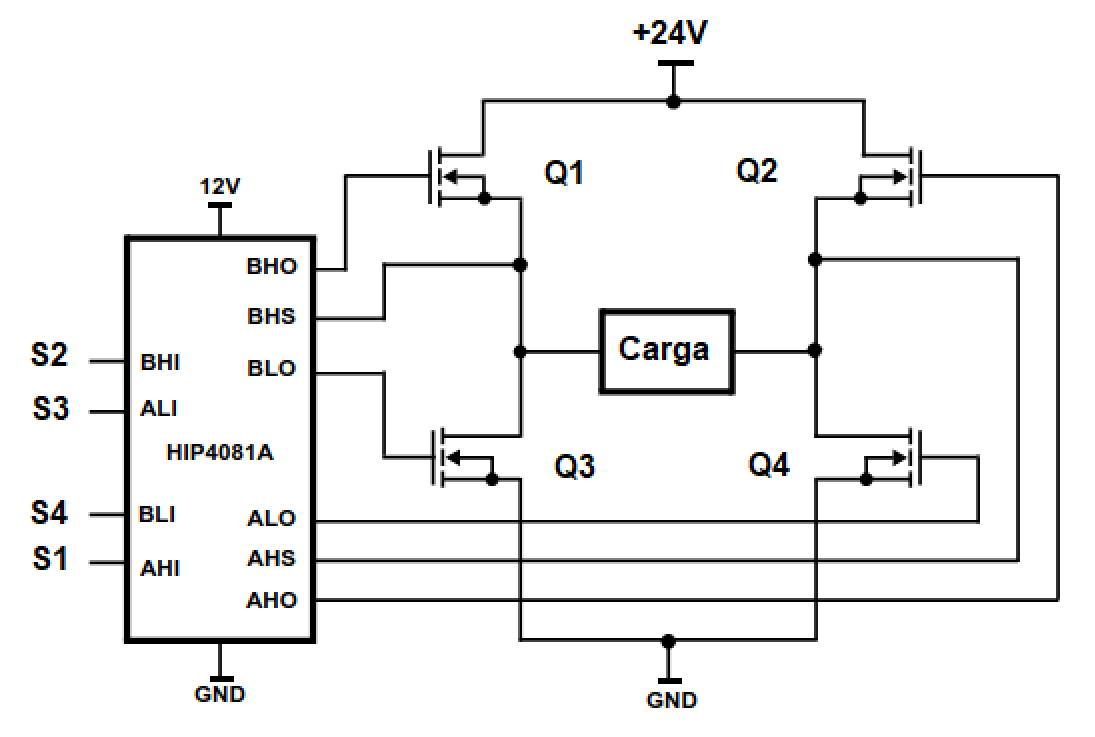
\includegraphics[scale=0.7]{Topologia-puenteH.png}
	\caption{Topología elemental del puente H.}
	\label{fig:img_topologia-puenteH}
\end{figure}
